
%(BEGIN_QUESTION)
% Copyright 2007, Tony R. Kuphaldt, released under the Creative Commons Attribution License (v 1.0)
% This means you may do almost anything with this work of mine, so long as you give me proper credit

Suppose we wished to implement a temperature controller with triple-redundant transmitters using FOUNDATION Fieldbus.  A general P\&ID of the control scheme is shown here:

$$\includegraphics[width=15.5cm]{i02445x02.eps}$$

The ``median select'' relay selects the temperature transmitter's signal that lies {\it between} the other two.  This way, neither a high-signal failure nor a low-signal failure in any one temperature transmitter will cause the temperature controller to take false action.  Any single transmitter failure will merely cause a maintenance alarm, and the control system will continue to act as it should.

\filbreak

There is more than one way to divide these functions among the various field instruments.  This Fieldbus function block diagram shows one way (note the italicized instrument tag names above each block):

$$\includegraphics[width=15.5cm]{i02445x01.eps}$$

With these function block assignments, the sequence of function block execution and Fieldbus data communication will look something like what is shown in this timing diagram:

$$\includegraphics[width=15.5cm]{i02445x03.eps}$$

Answer the following questions about this timing sequence:

\begin{itemize}
\item{} Identify the length of a {\it macrocycle} in the timing diagram.
\item{} Identify the purpose of each Compel Data (CD) token transmitted by the LAS.
\item{} Explain why there is no CD token transmitted by the LAS between the PID and AO function block execution times.
\item{} During what periods of time are unscheduled (acyclic) communications allowed to take place?
\item{} Do you see any way to reallocate any function blocks to different field devices to gain more reliability for the control system?
\end{itemize}

\underbar{file i02445}
%(END_QUESTION)





%(BEGIN_ANSWER)

\noindent
{\bf Partial answer:}

\begin{itemize}
\item{} Identify the length of a {\it macrocycle} in the timing diagram.  {\it The period the entire sequence takes to repeat: from thick bar to thick bar in the timing diagram.}
\vskip 5pt
\item{} Explain why there is no CD token transmitted by the LAS between the PID and AO function block execution times.  {\it Both blocks reside in the same field instrument and therefor do not need to communicate to each other over the bus.}
\vskip 5pt
\item{} Do you see any way to reallocate any function blocks to different field devices to gain more reliability for the control system?  {\it Sure!  (What??? You expect a detailed answer here?)}
\end{itemize}

%(END_ANSWER)





%(BEGIN_NOTES)

\begin{itemize}
\item{} Identify the length of a {\it macrocycle} in the timing diagram.  {\it The period the entire sequence takes to repeat: from thick bar to thick bar in the diagram.}
\vskip 5pt
\item{} Identify the purpose of each Compel Data (CD) token transmitted by the LAS.  {\it A CD is needed to tell each field device to transmit one of its function block output signals over the bus so function blocks in other devices can receive those signals.  Thus, two CD's are needed to compel temperature transmitters TT-101b and TT-101c to publish their AO signals, one at a time, so that the ISEL block in TT-101a can read them.  The CD after the ISEL function compels it to publish its output data to the bus so the PID function block (located in the control valve) can read it.}
\vskip 5pt
\item{} Explain why there is no CD token transmitted by the LAS between the PID and AO function block execution times.  {\it Both blocks reside in the same field instrument and therefor do not need to communicate to each other over the bus.}
\vskip 5pt
\item{} During what periods of time are unscheduled (acyclic) communications allowed to take place?  {\it During all the times between the Compel Data (CD) token transmissions.  Yes, acyclic communication can take place during function block execution!  In fact, this is the best time for unscheduled communication, because the function blocks are busy doing their thing(s).}
\vskip 5pt
\item{} Do you see any way to reallocate any function blocks to different field devices to gain more reliability for the control system?  {\it Relocate the input selector (ISEL) block from TT-101a to the control valve TV-101.  Right now, TT-101a is not really redundant.  If it fails, the ISEL block fails with it, regardless of how well the other two temperature transmitters are functioning.}
\end{itemize}

Configuration software for the host system (usually a Fieldbus-aware DCS) allows the engineer or technician to view the macrocycle and timing sequence.  Depending on how much freedom that host system software gives you to adjust the macrocycle details, your goal is to minimize macrocycle time while maximizing free (unscheduled) time within the macrocycle.  

Some host systems (example: Yokogawa) apply optimizing algorithms when configuring macrocycles.  For example, scheduling multiple cycles of execution for fast Fieldbus loops (``microcycles'') within each macrocycle, to achieve optimum response times for those fast loops.

\vfil \eject

\noindent
{\bf Summary Quiz:}

Explain why there is no CD token issued between the PID and AO function blocks in this macrocycle schedule:

$$\includegraphics[width=15.5cm]{i02445x03.eps}$$

\begin{itemize}
\item{} The device with the AO block is the backup LAS (backup Link Master)
\vskip 5pt 
\item{} These function blocks are both located inside the valve positioner (TV-101)
\vskip 5pt 
\item{} The BKCAL\_OUT signal has not been connected between these function blocks
\vskip 5pt 
\item{} Communication between PID and AO blocks is acyclic (unscheduled)
\vskip 5pt 
\item{} The AI and ISEL function blocks are both located inside transmitter TT-101a
\vskip 5pt 
\item{} The LAS has taken the device with the PID block off the Live List
\end{itemize}

%INDEX% Control, strategies: selector (using ISEL Fieldbus function block)
%INDEX% Fieldbus, function block: block execution sequence
%INDEX% Fieldbus, function block: macrocycle
%INDEX% Process: heater (fired) (generic)

%(END_NOTES)


